% Options for packages loaded elsewhere
\PassOptionsToPackage{unicode}{hyperref}
\PassOptionsToPackage{hyphens}{url}
%
\documentclass[
]{article}
\usepackage{amsmath,amssymb}
\usepackage{lmodern}
\usepackage{iftex}
\ifPDFTeX
  \usepackage[T1]{fontenc}
  \usepackage[utf8]{inputenc}
  \usepackage{textcomp} % provide euro and other symbols
\else % if luatex or xetex
  \usepackage{unicode-math}
  \defaultfontfeatures{Scale=MatchLowercase}
  \defaultfontfeatures[\rmfamily]{Ligatures=TeX,Scale=1}
\fi
% Use upquote if available, for straight quotes in verbatim environments
\IfFileExists{upquote.sty}{\usepackage{upquote}}{}
\IfFileExists{microtype.sty}{% use microtype if available
  \usepackage[]{microtype}
  \UseMicrotypeSet[protrusion]{basicmath} % disable protrusion for tt fonts
}{}
\makeatletter
\@ifundefined{KOMAClassName}{% if non-KOMA class
  \IfFileExists{parskip.sty}{%
    \usepackage{parskip}
  }{% else
    \setlength{\parindent}{0pt}
    \setlength{\parskip}{6pt plus 2pt minus 1pt}}
}{% if KOMA class
  \KOMAoptions{parskip=half}}
\makeatother
\usepackage{xcolor}
\IfFileExists{xurl.sty}{\usepackage{xurl}}{} % add URL line breaks if available
\IfFileExists{bookmark.sty}{\usepackage{bookmark}}{\usepackage{hyperref}}
\hypersetup{
  pdfauthor={Jeanne McClure},
  hidelinks,
  pdfcreator={LaTeX via pandoc}}
\urlstyle{same} % disable monospaced font for URLs
\usepackage[margin=1in]{geometry}
\usepackage{color}
\usepackage{fancyvrb}
\newcommand{\VerbBar}{|}
\newcommand{\VERB}{\Verb[commandchars=\\\{\}]}
\DefineVerbatimEnvironment{Highlighting}{Verbatim}{commandchars=\\\{\}}
% Add ',fontsize=\small' for more characters per line
\usepackage{framed}
\definecolor{shadecolor}{RGB}{248,248,248}
\newenvironment{Shaded}{\begin{snugshade}}{\end{snugshade}}
\newcommand{\AlertTok}[1]{\textcolor[rgb]{0.94,0.16,0.16}{#1}}
\newcommand{\AnnotationTok}[1]{\textcolor[rgb]{0.56,0.35,0.01}{\textbf{\textit{#1}}}}
\newcommand{\AttributeTok}[1]{\textcolor[rgb]{0.77,0.63,0.00}{#1}}
\newcommand{\BaseNTok}[1]{\textcolor[rgb]{0.00,0.00,0.81}{#1}}
\newcommand{\BuiltInTok}[1]{#1}
\newcommand{\CharTok}[1]{\textcolor[rgb]{0.31,0.60,0.02}{#1}}
\newcommand{\CommentTok}[1]{\textcolor[rgb]{0.56,0.35,0.01}{\textit{#1}}}
\newcommand{\CommentVarTok}[1]{\textcolor[rgb]{0.56,0.35,0.01}{\textbf{\textit{#1}}}}
\newcommand{\ConstantTok}[1]{\textcolor[rgb]{0.00,0.00,0.00}{#1}}
\newcommand{\ControlFlowTok}[1]{\textcolor[rgb]{0.13,0.29,0.53}{\textbf{#1}}}
\newcommand{\DataTypeTok}[1]{\textcolor[rgb]{0.13,0.29,0.53}{#1}}
\newcommand{\DecValTok}[1]{\textcolor[rgb]{0.00,0.00,0.81}{#1}}
\newcommand{\DocumentationTok}[1]{\textcolor[rgb]{0.56,0.35,0.01}{\textbf{\textit{#1}}}}
\newcommand{\ErrorTok}[1]{\textcolor[rgb]{0.64,0.00,0.00}{\textbf{#1}}}
\newcommand{\ExtensionTok}[1]{#1}
\newcommand{\FloatTok}[1]{\textcolor[rgb]{0.00,0.00,0.81}{#1}}
\newcommand{\FunctionTok}[1]{\textcolor[rgb]{0.00,0.00,0.00}{#1}}
\newcommand{\ImportTok}[1]{#1}
\newcommand{\InformationTok}[1]{\textcolor[rgb]{0.56,0.35,0.01}{\textbf{\textit{#1}}}}
\newcommand{\KeywordTok}[1]{\textcolor[rgb]{0.13,0.29,0.53}{\textbf{#1}}}
\newcommand{\NormalTok}[1]{#1}
\newcommand{\OperatorTok}[1]{\textcolor[rgb]{0.81,0.36,0.00}{\textbf{#1}}}
\newcommand{\OtherTok}[1]{\textcolor[rgb]{0.56,0.35,0.01}{#1}}
\newcommand{\PreprocessorTok}[1]{\textcolor[rgb]{0.56,0.35,0.01}{\textit{#1}}}
\newcommand{\RegionMarkerTok}[1]{#1}
\newcommand{\SpecialCharTok}[1]{\textcolor[rgb]{0.00,0.00,0.00}{#1}}
\newcommand{\SpecialStringTok}[1]{\textcolor[rgb]{0.31,0.60,0.02}{#1}}
\newcommand{\StringTok}[1]{\textcolor[rgb]{0.31,0.60,0.02}{#1}}
\newcommand{\VariableTok}[1]{\textcolor[rgb]{0.00,0.00,0.00}{#1}}
\newcommand{\VerbatimStringTok}[1]{\textcolor[rgb]{0.31,0.60,0.02}{#1}}
\newcommand{\WarningTok}[1]{\textcolor[rgb]{0.56,0.35,0.01}{\textbf{\textit{#1}}}}
\usepackage{longtable,booktabs,array}
\usepackage{calc} % for calculating minipage widths
% Correct order of tables after \paragraph or \subparagraph
\usepackage{etoolbox}
\makeatletter
\patchcmd\longtable{\par}{\if@noskipsec\mbox{}\fi\par}{}{}
\makeatother
% Allow footnotes in longtable head/foot
\IfFileExists{footnotehyper.sty}{\usepackage{footnotehyper}}{\usepackage{footnote}}
\makesavenoteenv{longtable}
\usepackage{graphicx}
\makeatletter
\def\maxwidth{\ifdim\Gin@nat@width>\linewidth\linewidth\else\Gin@nat@width\fi}
\def\maxheight{\ifdim\Gin@nat@height>\textheight\textheight\else\Gin@nat@height\fi}
\makeatother
% Scale images if necessary, so that they will not overflow the page
% margins by default, and it is still possible to overwrite the defaults
% using explicit options in \includegraphics[width, height, ...]{}
\setkeys{Gin}{width=\maxwidth,height=\maxheight,keepaspectratio}
% Set default figure placement to htbp
\makeatletter
\def\fps@figure{htbp}
\makeatother
\setlength{\emergencystretch}{3em} % prevent overfull lines
\providecommand{\tightlist}{%
  \setlength{\itemsep}{0pt}\setlength{\parskip}{0pt}}
\setcounter{secnumdepth}{-\maxdimen} % remove section numbering
\ifLuaTeX
  \usepackage{selnolig}  % disable illegal ligatures
\fi

\author{Jeanne McClure}
\date{2022-07-08}

\begin{document}

\hypertarget{introduction}{%
\subsection{0. Introduction}\label{introduction}}

Provide a brief overview or case study.

\begin{itemize}
\tightlist
\item
  Include your R1: \emph{research questions!}
\end{itemize}

\hypertarget{prepare}{%
\subsection{1. Prepare}\label{prepare}}

Load Packages

\begin{Shaded}
\begin{Highlighting}[]
\CommentTok{\#Load necessary packages}
\FunctionTok{library}\NormalTok{(tidyverse)}
\FunctionTok{library}\NormalTok{(here)}
\end{Highlighting}
\end{Shaded}

\hypertarget{wrangle}{%
\subsection{2. Wrangle}\label{wrangle}}

\hypertarget{a.-import-data}{%
\subsubsection{\texorpdfstring{a. \emph{Import
Data}}{a. Import Data}}\label{a.-import-data}}

\hypertarget{data-source-1-log-data}{%
\paragraph{Data Source \#1: Log Data}\label{data-source-1-log-data}}

Log-trace data is data generated from our interactions with digital
technologies, such as archived data from social media postings. In
education, an increasingly common source of log-trace data is that
generated from interactions with LMS and other digital tools.

The data we will use has already been ``wrangled'' quite a bit and is a
summary type of log-trace data: the number of minutes students spent on
the course. While this data type is fairly straightforward, there are
even more complex sources of log-trace data out there (e.g., time stamps
associated with when students started and stopped accessing the course).

Let's use the \texttt{read\_csv()} function from \{readr\} to import our
\texttt{log-data.csv} file directly from our data folder and name this
data set \texttt{time\_spent}, to help us to quickly recollect what
function it serves in this analysis:

\begin{Shaded}
\begin{Highlighting}[]
\CommentTok{\#load with read\_csv package}
\NormalTok{time\_spent }\OtherTok{\textless{}{-}} \FunctionTok{read\_csv}\NormalTok{(}\StringTok{"\textasciitilde{}/RProj22/foundation\_labs\_2022/foundation\_lab\_2/data/log{-}data.csv"}\NormalTok{)}
\end{Highlighting}
\end{Shaded}

\begin{verbatim}
## Rows: 716 Columns: 6
## -- Column specification --------------------------------------------------------
## Delimiter: ","
## chr (4): course_id, gender, enrollment_reason, enrollment_status
## dbl (2): student_id, time_spent
## 
## i Use `spec()` to retrieve the full column specification for this data.
## i Specify the column types or set `show_col_types = FALSE` to quiet this message.
\end{verbatim}

\begin{Shaded}
\begin{Highlighting}[]
\CommentTok{\#read in data\_to\_explore}
\NormalTok{data\_to\_explore }\OtherTok{\textless{}{-}} \FunctionTok{read\_csv}\NormalTok{(}\FunctionTok{here}\NormalTok{(}\StringTok{"data"}\NormalTok{, }\StringTok{"data\_to\_explore.csv"}\NormalTok{))}
\end{Highlighting}
\end{Shaded}

\begin{verbatim}
## Rows: 943 Columns: 34
## -- Column specification --------------------------------------------------------
## Delimiter: ","
## chr   (8): student_id, subject, semester, section, gender, enrollment_reason...
## dbl  (23): total_points_possible, total_points_earned, proportion_earned, ti...
## dttm  (3): date_x, date_y, date
## 
## i Use `spec()` to retrieve the full column specification for this data.
## i Specify the column types or set `show_col_types = FALSE` to quiet this message.
\end{verbatim}

\hypertarget{explore}{%
\subsection{3. Explore}\label{explore}}

\hypertarget{a.-table-summary}{%
\paragraph{A. TABLE SUMMARY}\label{a.-table-summary}}

\begin{Shaded}
\begin{Highlighting}[]
\CommentTok{\#install package if this is first time using skimr}


\CommentTok{\#load library}
\FunctionTok{library}\NormalTok{(skimr)}

\CommentTok{\#skim data}
\FunctionTok{skim}\NormalTok{(data\_to\_explore)}
\end{Highlighting}
\end{Shaded}

\begin{longtable}[]{@{}ll@{}}
\caption{Data summary}\tabularnewline
\toprule
\endhead
Name & data\_to\_explore \\
Number of rows & 943 \\
Number of columns & 34 \\
\_\_\_\_\_\_\_\_\_\_\_\_\_\_\_\_\_\_\_\_\_\_\_ & \\
Column type frequency: & \\
character & 8 \\
numeric & 23 \\
POSIXct & 3 \\
\_\_\_\_\_\_\_\_\_\_\_\_\_\_\_\_\_\_\_\_\_\_\_\_ & \\
Group variables & None \\
\bottomrule
\end{longtable}

\textbf{Variable type: character}

\begin{longtable}[]{@{}
  >{\raggedright\arraybackslash}p{(\columnwidth - 14\tabcolsep) * \real{0.2368}}
  >{\raggedleft\arraybackslash}p{(\columnwidth - 14\tabcolsep) * \real{0.1316}}
  >{\raggedleft\arraybackslash}p{(\columnwidth - 14\tabcolsep) * \real{0.1842}}
  >{\raggedleft\arraybackslash}p{(\columnwidth - 14\tabcolsep) * \real{0.0526}}
  >{\raggedleft\arraybackslash}p{(\columnwidth - 14\tabcolsep) * \real{0.0526}}
  >{\raggedleft\arraybackslash}p{(\columnwidth - 14\tabcolsep) * \real{0.0789}}
  >{\raggedleft\arraybackslash}p{(\columnwidth - 14\tabcolsep) * \real{0.1184}}
  >{\raggedleft\arraybackslash}p{(\columnwidth - 14\tabcolsep) * \real{0.1447}}@{}}
\toprule
\begin{minipage}[b]{\linewidth}\raggedright
skim\_variable
\end{minipage} & \begin{minipage}[b]{\linewidth}\raggedleft
n\_missing
\end{minipage} & \begin{minipage}[b]{\linewidth}\raggedleft
complete\_rate
\end{minipage} & \begin{minipage}[b]{\linewidth}\raggedleft
min
\end{minipage} & \begin{minipage}[b]{\linewidth}\raggedleft
max
\end{minipage} & \begin{minipage}[b]{\linewidth}\raggedleft
empty
\end{minipage} & \begin{minipage}[b]{\linewidth}\raggedleft
n\_unique
\end{minipage} & \begin{minipage}[b]{\linewidth}\raggedleft
whitespace
\end{minipage} \\
\midrule
\endhead
student\_id & 0 & 1.00 & 2 & 6 & 0 & 879 & 0 \\
subject & 0 & 1.00 & 4 & 5 & 0 & 5 & 0 \\
semester & 0 & 1.00 & 4 & 4 & 0 & 4 & 0 \\
section & 0 & 1.00 & 2 & 2 & 0 & 4 & 0 \\
gender & 227 & 0.76 & 1 & 1 & 0 & 2 & 0 \\
enrollment\_reason & 227 & 0.76 & 5 & 34 & 0 & 5 & 0 \\
enrollment\_status & 227 & 0.76 & 7 & 17 & 0 & 3 & 0 \\
course\_id & 281 & 0.70 & 12 & 13 & 0 & 36 & 0 \\
\bottomrule
\end{longtable}

\textbf{Variable type: numeric}

\begin{longtable}[]{@{}
  >{\raggedright\arraybackslash}p{(\columnwidth - 20\tabcolsep) * \real{0.2037}}
  >{\raggedleft\arraybackslash}p{(\columnwidth - 20\tabcolsep) * \real{0.0926}}
  >{\raggedleft\arraybackslash}p{(\columnwidth - 20\tabcolsep) * \real{0.1296}}
  >{\raggedleft\arraybackslash}p{(\columnwidth - 20\tabcolsep) * \real{0.0741}}
  >{\raggedleft\arraybackslash}p{(\columnwidth - 20\tabcolsep) * \real{0.0741}}
  >{\raggedleft\arraybackslash}p{(\columnwidth - 20\tabcolsep) * \real{0.0741}}
  >{\raggedleft\arraybackslash}p{(\columnwidth - 20\tabcolsep) * \real{0.0741}}
  >{\raggedleft\arraybackslash}p{(\columnwidth - 20\tabcolsep) * \real{0.0741}}
  >{\raggedleft\arraybackslash}p{(\columnwidth - 20\tabcolsep) * \real{0.0741}}
  >{\raggedleft\arraybackslash}p{(\columnwidth - 20\tabcolsep) * \real{0.0741}}
  >{\raggedright\arraybackslash}p{(\columnwidth - 20\tabcolsep) * \real{0.0556}}@{}}
\toprule
\begin{minipage}[b]{\linewidth}\raggedright
skim\_variable
\end{minipage} & \begin{minipage}[b]{\linewidth}\raggedleft
n\_missing
\end{minipage} & \begin{minipage}[b]{\linewidth}\raggedleft
complete\_rate
\end{minipage} & \begin{minipage}[b]{\linewidth}\raggedleft
mean
\end{minipage} & \begin{minipage}[b]{\linewidth}\raggedleft
sd
\end{minipage} & \begin{minipage}[b]{\linewidth}\raggedleft
p0
\end{minipage} & \begin{minipage}[b]{\linewidth}\raggedleft
p25
\end{minipage} & \begin{minipage}[b]{\linewidth}\raggedleft
p50
\end{minipage} & \begin{minipage}[b]{\linewidth}\raggedleft
p75
\end{minipage} & \begin{minipage}[b]{\linewidth}\raggedleft
p100
\end{minipage} & \begin{minipage}[b]{\linewidth}\raggedright
hist
\end{minipage} \\
\midrule
\endhead
total\_points\_possible & 226 & 0.76 & 1619.55 & 387.12 & 1212.00 &
1217.00 & 1676.00 & 1791.00 & 2425.00 & ▇▂▆▁▃ \\
total\_points\_earned & 226 & 0.76 & 1229.98 & 510.64 & 0.00 & 1002.50 &
1177.13 & 1572.45 & 2413.50 & ▂▂▇▅▂ \\
proportion\_earned & 226 & 0.76 & 0.76 & 0.25 & 0.00 & 0.72 & 0.86 &
0.92 & 1.01 & ▁▁▁▃▇ \\
time\_spent & 232 & 0.75 & 1828.80 & 1363.13 & 0.45 & 895.57 & 1559.97 &
2423.94 & 8870.88 & ▇▅▁▁▁ \\
time\_spent\_hours & 232 & 0.75 & 30.48 & 22.72 & 0.01 & 14.93 & 26.00 &
40.40 & 147.85 & ▇▅▁▁▁ \\
int & 293 & 0.69 & 4.30 & 0.60 & 1.80 & 4.00 & 4.40 & 4.80 & 5.00 &
▁▁▂▆▇ \\
val & 287 & 0.70 & 3.75 & 0.75 & 1.00 & 3.33 & 3.67 & 4.33 & 5.00 &
▁▁▆▇▆ \\
percomp & 288 & 0.69 & 3.64 & 0.69 & 1.50 & 3.00 & 3.50 & 4.00 & 5.00 &
▁▁▇▃▃ \\
tv & 292 & 0.69 & 4.07 & 0.59 & 1.00 & 3.71 & 4.12 & 4.46 & 5.00 &
▁▁▂▇▇ \\
q1 & 285 & 0.70 & 4.34 & 0.66 & 1.00 & 4.00 & 4.00 & 5.00 & 5.00 &
▁▁▁▇▇ \\
q2 & 285 & 0.70 & 3.66 & 0.93 & 1.00 & 3.00 & 4.00 & 4.00 & 5.00 &
▁▂▆▇▃ \\
q3 & 286 & 0.70 & 3.31 & 0.85 & 1.00 & 3.00 & 3.00 & 4.00 & 5.00 &
▁▂▇▅▂ \\
q4 & 289 & 0.69 & 4.35 & 0.80 & 1.00 & 4.00 & 5.00 & 5.00 & 5.00 &
▁▁▁▆▇ \\
q5 & 286 & 0.70 & 4.28 & 0.69 & 1.00 & 4.00 & 4.00 & 5.00 & 5.00 &
▁▁▁▇▆ \\
q6 & 285 & 0.70 & 4.05 & 0.80 & 1.00 & 4.00 & 4.00 & 5.00 & 5.00 &
▁▁▃▇▅ \\
q7 & 286 & 0.70 & 3.96 & 0.85 & 1.00 & 3.00 & 4.00 & 5.00 & 5.00 &
▁▁▅▇▆ \\
q8 & 286 & 0.70 & 4.35 & 0.65 & 1.00 & 4.00 & 4.00 & 5.00 & 5.00 &
▁▁▁▇▇ \\
q9 & 286 & 0.70 & 3.55 & 0.92 & 1.00 & 3.00 & 4.00 & 4.00 & 5.00 &
▁▂▇▇▃ \\
q10 & 285 & 0.70 & 4.17 & 0.87 & 1.00 & 4.00 & 4.00 & 5.00 & 5.00 &
▁▁▃▇▇ \\
post\_int & 848 & 0.10 & 3.88 & 0.94 & 1.00 & 3.50 & 4.00 & 4.50 & 5.00
& ▁▁▃▇▇ \\
post\_uv & 848 & 0.10 & 3.48 & 0.99 & 1.00 & 3.00 & 3.67 & 4.00 & 5.00 &
▂▂▅▇▅ \\
post\_tv & 848 & 0.10 & 3.71 & 0.90 & 1.00 & 3.29 & 3.86 & 4.29 & 5.00 &
▁▂▃▇▆ \\
post\_percomp & 848 & 0.10 & 3.47 & 0.88 & 1.00 & 3.00 & 3.50 & 4.00 &
5.00 & ▁▂▂▇▂ \\
\bottomrule
\end{longtable}

\textbf{Variable type: POSIXct}

\begin{longtable}[]{@{}
  >{\raggedright\arraybackslash}p{(\columnwidth - 12\tabcolsep) * \real{0.1308}}
  >{\raggedleft\arraybackslash}p{(\columnwidth - 12\tabcolsep) * \real{0.0935}}
  >{\raggedleft\arraybackslash}p{(\columnwidth - 12\tabcolsep) * \real{0.1308}}
  >{\raggedright\arraybackslash}p{(\columnwidth - 12\tabcolsep) * \real{0.1869}}
  >{\raggedright\arraybackslash}p{(\columnwidth - 12\tabcolsep) * \real{0.1869}}
  >{\raggedright\arraybackslash}p{(\columnwidth - 12\tabcolsep) * \real{0.1869}}
  >{\raggedleft\arraybackslash}p{(\columnwidth - 12\tabcolsep) * \real{0.0841}}@{}}
\toprule
\begin{minipage}[b]{\linewidth}\raggedright
skim\_variable
\end{minipage} & \begin{minipage}[b]{\linewidth}\raggedleft
n\_missing
\end{minipage} & \begin{minipage}[b]{\linewidth}\raggedleft
complete\_rate
\end{minipage} & \begin{minipage}[b]{\linewidth}\raggedright
min
\end{minipage} & \begin{minipage}[b]{\linewidth}\raggedright
max
\end{minipage} & \begin{minipage}[b]{\linewidth}\raggedright
median
\end{minipage} & \begin{minipage}[b]{\linewidth}\raggedleft
n\_unique
\end{minipage} \\
\midrule
\endhead
date\_x & 393 & 0.58 & 2015-09-02 15:40:00 & 2016-05-24 15:53:00 &
2015-10-01 15:57:30 & 536 \\
date\_y & 848 & 0.10 & 2015-09-02 15:31:00 & 2016-01-22 15:43:00 &
2016-01-04 13:25:00 & 95 \\
date & 834 & 0.12 & 2017-01-23 13:14:00 & 2017-02-13 13:00:00 &
2017-01-25 18:43:00 & 107 \\
\bottomrule
\end{longtable}

\hypertarget{b.-tidy-to-explore}{%
\subsection{B. TIDY to EXPLORE}\label{b.-tidy-to-explore}}

\begin{Shaded}
\begin{Highlighting}[]
\CommentTok{\# using the \textasciigrave{}select()\textasciigrave{} and \textasciigrave{}filter()\textasciigrave{} functions. In the code chunk below,look at descriptive for just \textasciigrave{}proportion\_earned\textasciigrave{} , \textasciigrave{}time\_spent\textasciigrave{} and \textasciigrave{}gender\textasciigrave{}, but only for the "OcnA" and "PhysA" subjects.}

\NormalTok{data\_to\_explore }\SpecialCharTok{\%\textgreater{}\%} 
  \FunctionTok{select}\NormalTok{(}\FunctionTok{c}\NormalTok{(}\StringTok{\textquotesingle{}subject\textquotesingle{}}\NormalTok{, }\StringTok{\textquotesingle{}gender\textquotesingle{}}\NormalTok{, }\StringTok{\textquotesingle{}proportion\_earned\textquotesingle{}}\NormalTok{, }\StringTok{\textquotesingle{}time\_spent\textquotesingle{}}\NormalTok{)) }\SpecialCharTok{\%\textgreater{}\%} 
  \FunctionTok{filter}\NormalTok{(subject }\SpecialCharTok{==} \StringTok{"OcnA"} \SpecialCharTok{|}\NormalTok{ subject }\SpecialCharTok{==} \StringTok{"PhysA"}\NormalTok{) }\SpecialCharTok{\%\textgreater{}\%}
  \FunctionTok{skim}\NormalTok{()}
\end{Highlighting}
\end{Shaded}

\begin{longtable}[]{@{}ll@{}}
\caption{Data summary}\tabularnewline
\toprule
\endhead
Name & Piped data \\
Number of rows & 249 \\
Number of columns & 4 \\
\_\_\_\_\_\_\_\_\_\_\_\_\_\_\_\_\_\_\_\_\_\_\_ & \\
Column type frequency: & \\
character & 2 \\
numeric & 2 \\
\_\_\_\_\_\_\_\_\_\_\_\_\_\_\_\_\_\_\_\_\_\_\_\_ & \\
Group variables & None \\
\bottomrule
\end{longtable}

\textbf{Variable type: character}

\begin{longtable}[]{@{}
  >{\raggedright\arraybackslash}p{(\columnwidth - 14\tabcolsep) * \real{0.1944}}
  >{\raggedleft\arraybackslash}p{(\columnwidth - 14\tabcolsep) * \real{0.1389}}
  >{\raggedleft\arraybackslash}p{(\columnwidth - 14\tabcolsep) * \real{0.1944}}
  >{\raggedleft\arraybackslash}p{(\columnwidth - 14\tabcolsep) * \real{0.0556}}
  >{\raggedleft\arraybackslash}p{(\columnwidth - 14\tabcolsep) * \real{0.0556}}
  >{\raggedleft\arraybackslash}p{(\columnwidth - 14\tabcolsep) * \real{0.0833}}
  >{\raggedleft\arraybackslash}p{(\columnwidth - 14\tabcolsep) * \real{0.1250}}
  >{\raggedleft\arraybackslash}p{(\columnwidth - 14\tabcolsep) * \real{0.1528}}@{}}
\toprule
\begin{minipage}[b]{\linewidth}\raggedright
skim\_variable
\end{minipage} & \begin{minipage}[b]{\linewidth}\raggedleft
n\_missing
\end{minipage} & \begin{minipage}[b]{\linewidth}\raggedleft
complete\_rate
\end{minipage} & \begin{minipage}[b]{\linewidth}\raggedleft
min
\end{minipage} & \begin{minipage}[b]{\linewidth}\raggedleft
max
\end{minipage} & \begin{minipage}[b]{\linewidth}\raggedleft
empty
\end{minipage} & \begin{minipage}[b]{\linewidth}\raggedleft
n\_unique
\end{minipage} & \begin{minipage}[b]{\linewidth}\raggedleft
whitespace
\end{minipage} \\
\midrule
\endhead
subject & 0 & 1.00 & 4 & 5 & 0 & 2 & 0 \\
gender & 48 & 0.81 & 1 & 1 & 0 & 2 & 0 \\
\bottomrule
\end{longtable}

\textbf{Variable type: numeric}

\begin{longtable}[]{@{}
  >{\raggedright\arraybackslash}p{(\columnwidth - 20\tabcolsep) * \real{0.1800}}
  >{\raggedleft\arraybackslash}p{(\columnwidth - 20\tabcolsep) * \real{0.1000}}
  >{\raggedleft\arraybackslash}p{(\columnwidth - 20\tabcolsep) * \real{0.1400}}
  >{\raggedleft\arraybackslash}p{(\columnwidth - 20\tabcolsep) * \real{0.0800}}
  >{\raggedleft\arraybackslash}p{(\columnwidth - 20\tabcolsep) * \real{0.0800}}
  >{\raggedleft\arraybackslash}p{(\columnwidth - 20\tabcolsep) * \real{0.0500}}
  >{\raggedleft\arraybackslash}p{(\columnwidth - 20\tabcolsep) * \real{0.0700}}
  >{\raggedleft\arraybackslash}p{(\columnwidth - 20\tabcolsep) * \real{0.0800}}
  >{\raggedleft\arraybackslash}p{(\columnwidth - 20\tabcolsep) * \real{0.0800}}
  >{\raggedleft\arraybackslash}p{(\columnwidth - 20\tabcolsep) * \real{0.0800}}
  >{\raggedright\arraybackslash}p{(\columnwidth - 20\tabcolsep) * \real{0.0600}}@{}}
\toprule
\begin{minipage}[b]{\linewidth}\raggedright
skim\_variable
\end{minipage} & \begin{minipage}[b]{\linewidth}\raggedleft
n\_missing
\end{minipage} & \begin{minipage}[b]{\linewidth}\raggedleft
complete\_rate
\end{minipage} & \begin{minipage}[b]{\linewidth}\raggedleft
mean
\end{minipage} & \begin{minipage}[b]{\linewidth}\raggedleft
sd
\end{minipage} & \begin{minipage}[b]{\linewidth}\raggedleft
p0
\end{minipage} & \begin{minipage}[b]{\linewidth}\raggedleft
p25
\end{minipage} & \begin{minipage}[b]{\linewidth}\raggedleft
p50
\end{minipage} & \begin{minipage}[b]{\linewidth}\raggedleft
p75
\end{minipage} & \begin{minipage}[b]{\linewidth}\raggedleft
p100
\end{minipage} & \begin{minipage}[b]{\linewidth}\raggedright
hist
\end{minipage} \\
\midrule
\endhead
proportion\_earned & 48 & 0.81 & 0.78 & 0.24 & 0.00 & 0.73 & 0.86 & 0.94
& 1.00 & ▁▁▁▃▇ \\
time\_spent & 48 & 0.81 & 1828.56 & 1374.13 & 0.58 & 943.07 & 1601.13 &
2356.88 & 8870.88 & ▇▅▁▁▁ \\
\bottomrule
\end{longtable}

\hypertarget{b.-data-viz}{%
\paragraph{B. DATA VIZ}\label{b.-data-viz}}

ggplot grammar - with layers

\hypertarget{layers---scatter-plot}{%
\subparagraph{layers - Scatter Plot}\label{layers---scatter-plot}}

Basic graph 1. data 2. aes 3. geom

\begin{Shaded}
\begin{Highlighting}[]
\CommentTok{\#layer 1: add data and aesthetics mapping }
\FunctionTok{ggplot}\NormalTok{(data\_to\_explore, }\CommentTok{\#\textless{}\textless{}}
       \FunctionTok{aes}\NormalTok{(}\AttributeTok{x =}\NormalTok{ time\_spent\_hours, }
           \AttributeTok{y =}\NormalTok{ proportion\_earned)) }\SpecialCharTok{+}
\CommentTok{\#layer 2: +  geom function type}
  \FunctionTok{geom\_point}\NormalTok{() }\CommentTok{\#\textless{}\textless{}}
\end{Highlighting}
\end{Shaded}

\begin{verbatim}
## Warning: Removed 345 rows containing missing values (geom_point).
\end{verbatim}

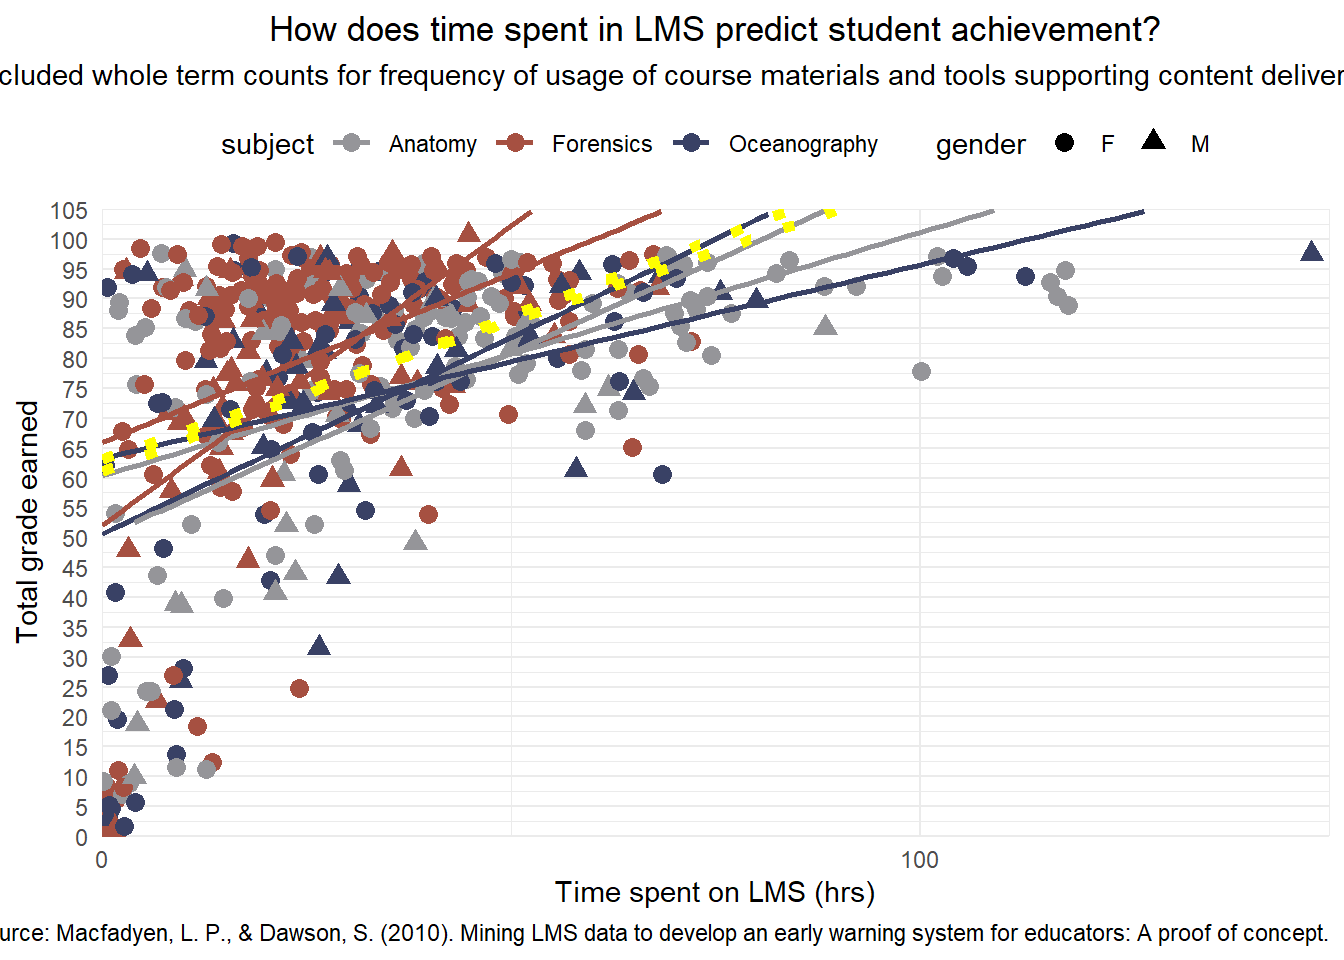
\includegraphics{final_pdf_files/figure-latex/unnamed-chunk-5-1.pdf}

Add \textbf{Scale } with different color for enrollment status.

\begin{Shaded}
\begin{Highlighting}[]
\CommentTok{\#layer 1: add data and aesthetics mapping }
\CommentTok{\#layer 3: add color scale by type}
\FunctionTok{ggplot}\NormalTok{(data\_to\_explore, }
       \FunctionTok{aes}\NormalTok{(}\AttributeTok{x =}\NormalTok{ time\_spent\_hours, }
           \AttributeTok{y =}\NormalTok{ proportion\_earned,}
           \AttributeTok{color =}\NormalTok{ enrollment\_status)) }\SpecialCharTok{+} \CommentTok{\#\textless{}\textless{}}
\CommentTok{\#layer 2: +  geom function type}
  \FunctionTok{geom\_point}\NormalTok{()}
\end{Highlighting}
\end{Shaded}

\begin{verbatim}
## Warning: Removed 345 rows containing missing values (geom_point).
\end{verbatim}

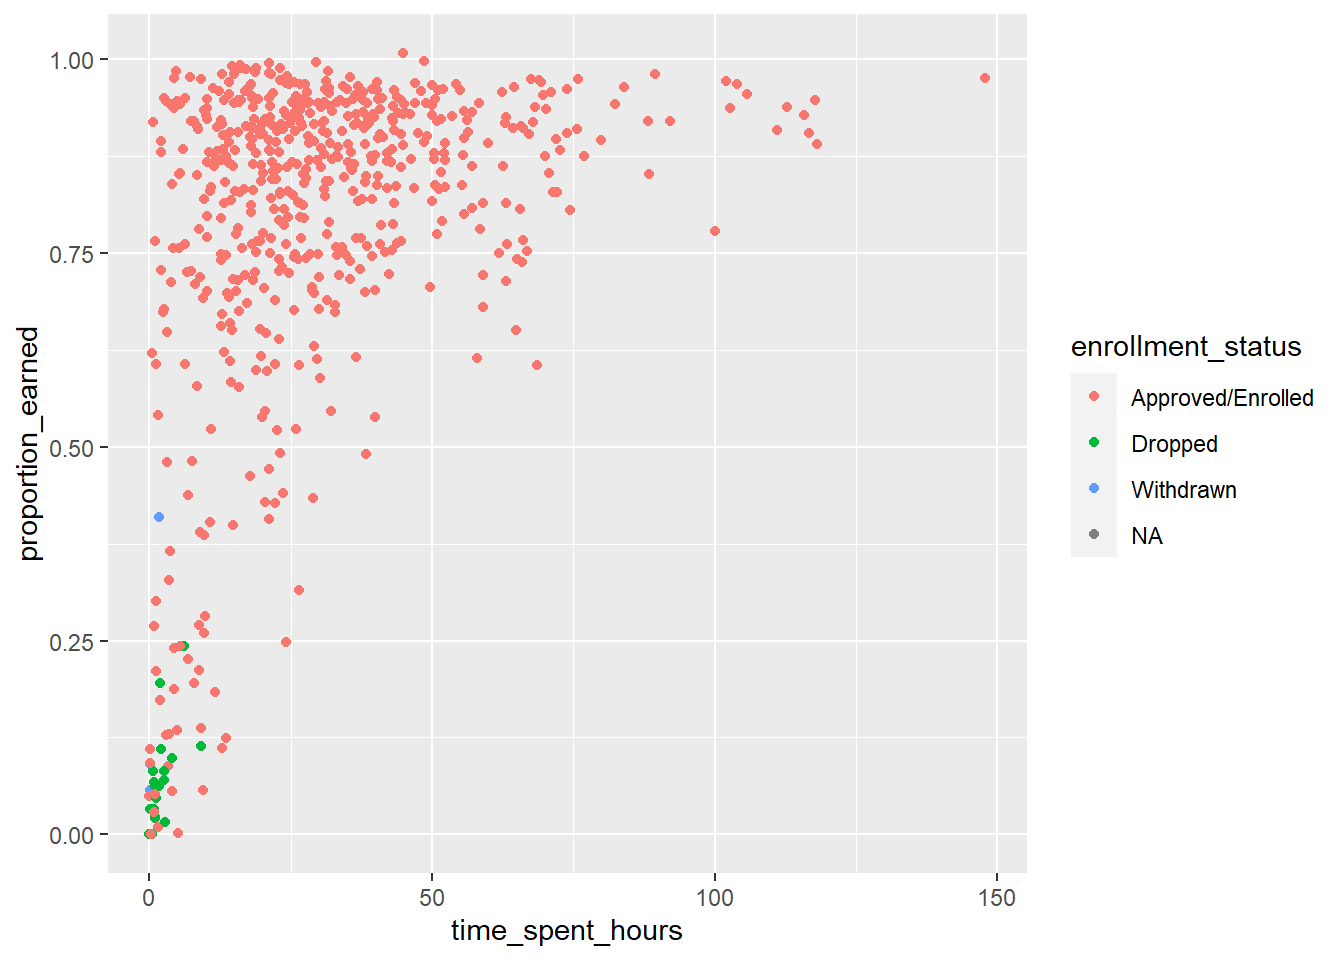
\includegraphics{final_pdf_files/figure-latex/unnamed-chunk-6-1.pdf}

Add another layer with **labs* labeling the title

\begin{Shaded}
\begin{Highlighting}[]
\CommentTok{\#layer 1: add data and aesthetics mapping }
\CommentTok{\#layer 3: add color scale by type}
\FunctionTok{ggplot}\NormalTok{(data\_to\_explore, }
       \FunctionTok{aes}\NormalTok{(}\AttributeTok{x =}\NormalTok{ time\_spent\_hours, }
           \AttributeTok{y =}\NormalTok{ proportion\_earned,}
           \AttributeTok{color =}\NormalTok{ enrollment\_status)) }\SpecialCharTok{+}
\CommentTok{\#layer 2: +  geom function type}
  \FunctionTok{geom\_point}\NormalTok{() }\SpecialCharTok{+}
\CommentTok{\#layer 4: add lables}
  \FunctionTok{labs}\NormalTok{(}\AttributeTok{title=}\StringTok{"How Time Spent on Course LMS is Related to Points Earned in the Course"}\NormalTok{, }\AttributeTok{x=}\StringTok{"Time Spent (Hours)"}\NormalTok{, }\AttributeTok{y =} \StringTok{"Proportion of Points Earned"}\NormalTok{)}
\end{Highlighting}
\end{Shaded}

\begin{verbatim}
## Warning: Removed 345 rows containing missing values (geom_point).
\end{verbatim}

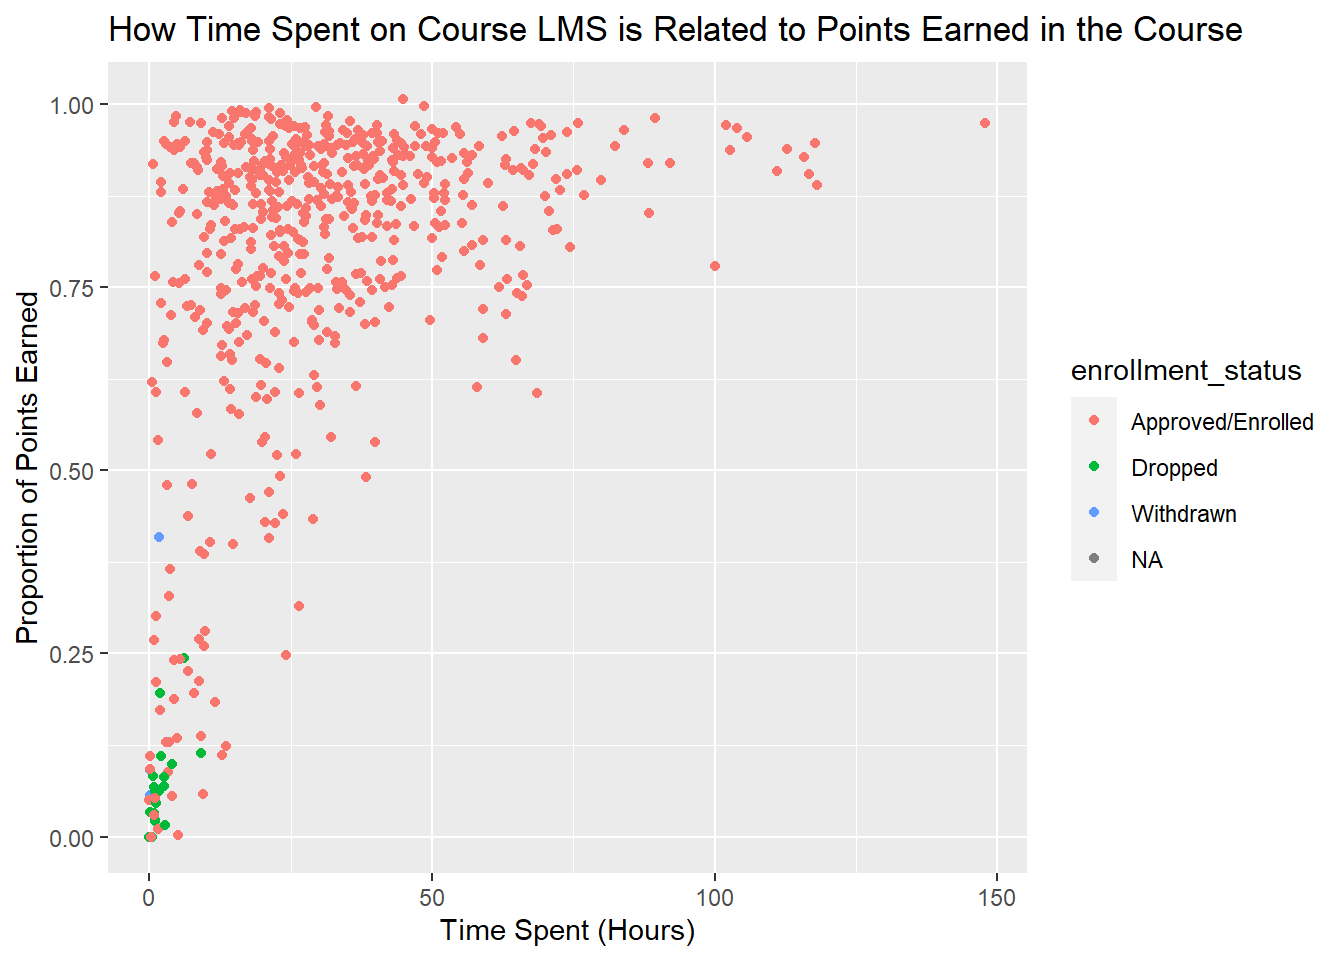
\includegraphics{final_pdf_files/figure-latex/unnamed-chunk-7-1.pdf}

Add the \textbf{facet} layer

\begin{Shaded}
\begin{Highlighting}[]
\CommentTok{\#layer 1: add data and aesthetics mapping }
\CommentTok{\#layer 3: add color scale by type}
\FunctionTok{ggplot}\NormalTok{(data\_to\_explore, }\FunctionTok{aes}\NormalTok{(}\AttributeTok{x =}\NormalTok{ time\_spent\_hours, }\AttributeTok{y =}\NormalTok{ proportion\_earned, }\AttributeTok{color =}\NormalTok{ enrollment\_status)) }\SpecialCharTok{+}
\CommentTok{\#layer 2: +  geom function type}
  \FunctionTok{geom\_point}\NormalTok{() }\SpecialCharTok{+}
\CommentTok{\#layer 4: add lables}
    \FunctionTok{x\_lab}\NormalTok{(}\AttributeTok{title=}\StringTok{"How Time Spent on Course LMS is Related to Points Earned in the Course"}\NormalTok{, }
       \AttributeTok{x=}\StringTok{"Time Spent (Hours)"}\NormalTok{,}
       \AttributeTok{y =} \StringTok{"Proportion of Points Earned"}\NormalTok{)}
\CommentTok{\#layer 5: add facet wrap}
  \FunctionTok{facet\_wrap}\NormalTok{(}\SpecialCharTok{\textasciitilde{}}\NormalTok{ subject) }
\end{Highlighting}
\end{Shaded}

\hypertarget{layers--histogram}{%
\subparagraph{layers- Histogram}\label{layers--histogram}}

Create a basic histogram using the `geom\_hist()' function

\begin{Shaded}
\begin{Highlighting}[]
\CommentTok{\# Layer 1: add data and aesthetic mapping}
\NormalTok{data\_to\_explore }\SpecialCharTok{\%\textgreater{}\%} \CommentTok{\#\textless{}\textless{}}
  \FunctionTok{ggplot}\NormalTok{(}\FunctionTok{aes}\NormalTok{(}\AttributeTok{x =}\NormalTok{ time\_spent\_hours)) }\SpecialCharTok{+}
\CommentTok{\# layer 2: add histogram geom}
  \FunctionTok{geom\_histogram}\NormalTok{()}
\end{Highlighting}
\end{Shaded}

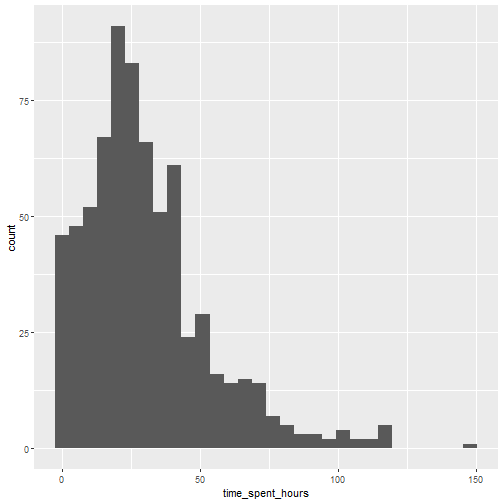
\includegraphics{final_pdf_files/figure-latex/hist1-1.pdf}

Change bin size

\begin{Shaded}
\begin{Highlighting}[]
\CommentTok{\# Layer 1: add data and aesthetic mapping}
\NormalTok{data\_to\_explore }\SpecialCharTok{\%\textgreater{}\%} 
  \FunctionTok{ggplot}\NormalTok{(}\FunctionTok{aes}\NormalTok{(}\AttributeTok{x =}\NormalTok{ time\_spent\_hours)) }\SpecialCharTok{+}
\CommentTok{\# layer 2: add histogram geom }
\CommentTok{\# layer 3a: add bin size}
  \FunctionTok{geom\_histogram}\NormalTok{(}\AttributeTok{bins =} \DecValTok{10}\NormalTok{)}
\end{Highlighting}
\end{Shaded}

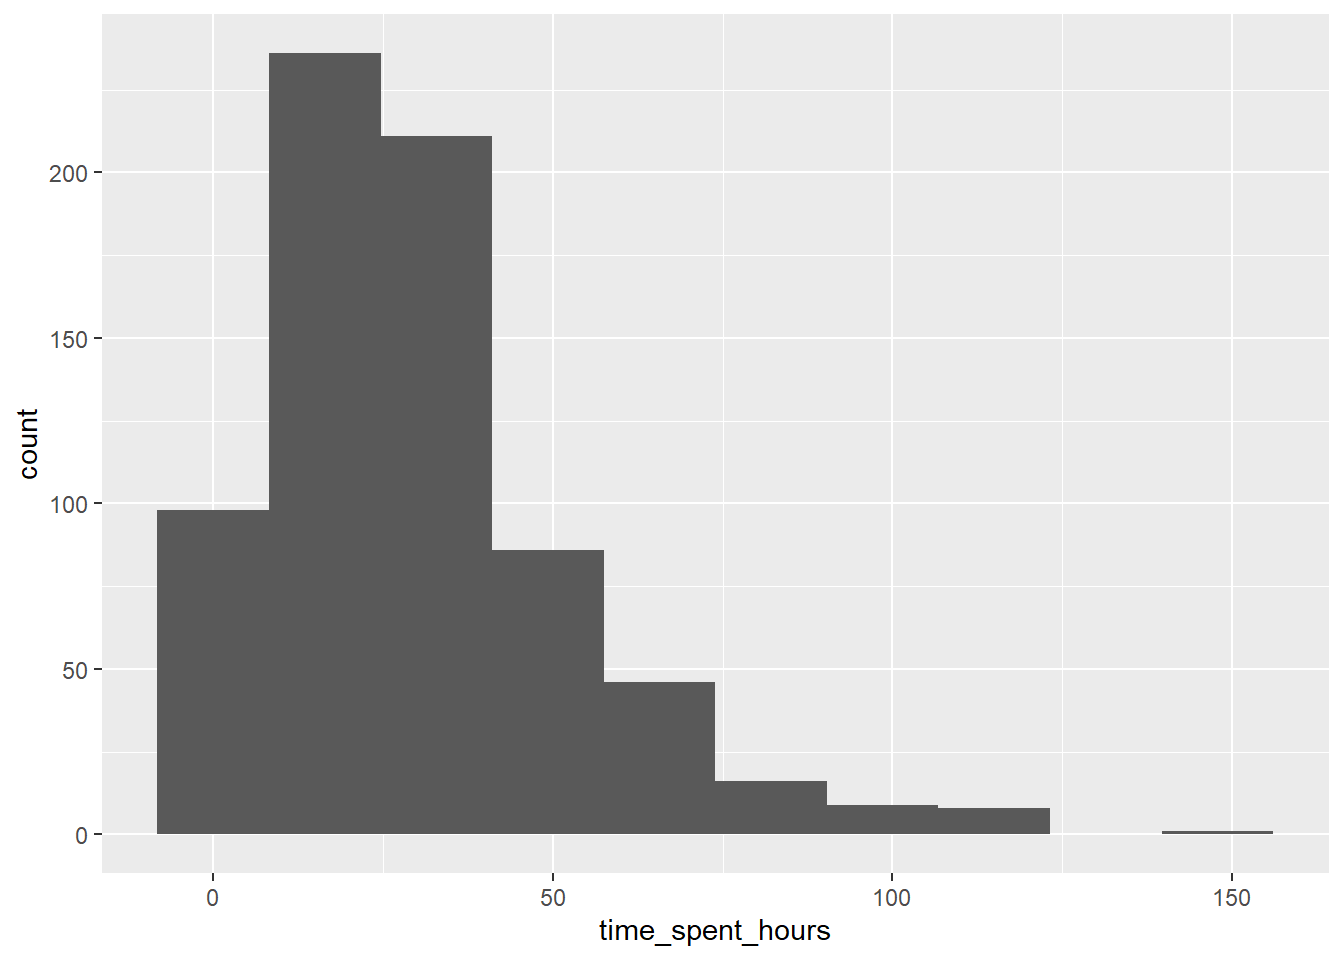
\includegraphics{final_pdf_files/figure-latex/hist2-1.pdf}

Add color label to make bins stand out

\begin{Shaded}
\begin{Highlighting}[]
\CommentTok{\# Layer 1: add data and aesthetic mapping}
\NormalTok{data\_to\_explore }\SpecialCharTok{\%\textgreater{}\%} 
  \FunctionTok{ggplot}\NormalTok{(}\FunctionTok{aes}\NormalTok{(}\AttributeTok{x =}\NormalTok{ time\_spent\_hours)) }\SpecialCharTok{+}
\CommentTok{\# layer 2: add histogram geom }
\CommentTok{\# layer 3a: add bin size}
\CommentTok{\#layer 3b: add color}
  \FunctionTok{geom\_histogram}\NormalTok{(}\AttributeTok{bins =} \DecValTok{10}\NormalTok{,}
                 \AttributeTok{fill =} \StringTok{"red"}\NormalTok{, }
                 \AttributeTok{colour =} \StringTok{"black"}\NormalTok{) }
\end{Highlighting}
\end{Shaded}

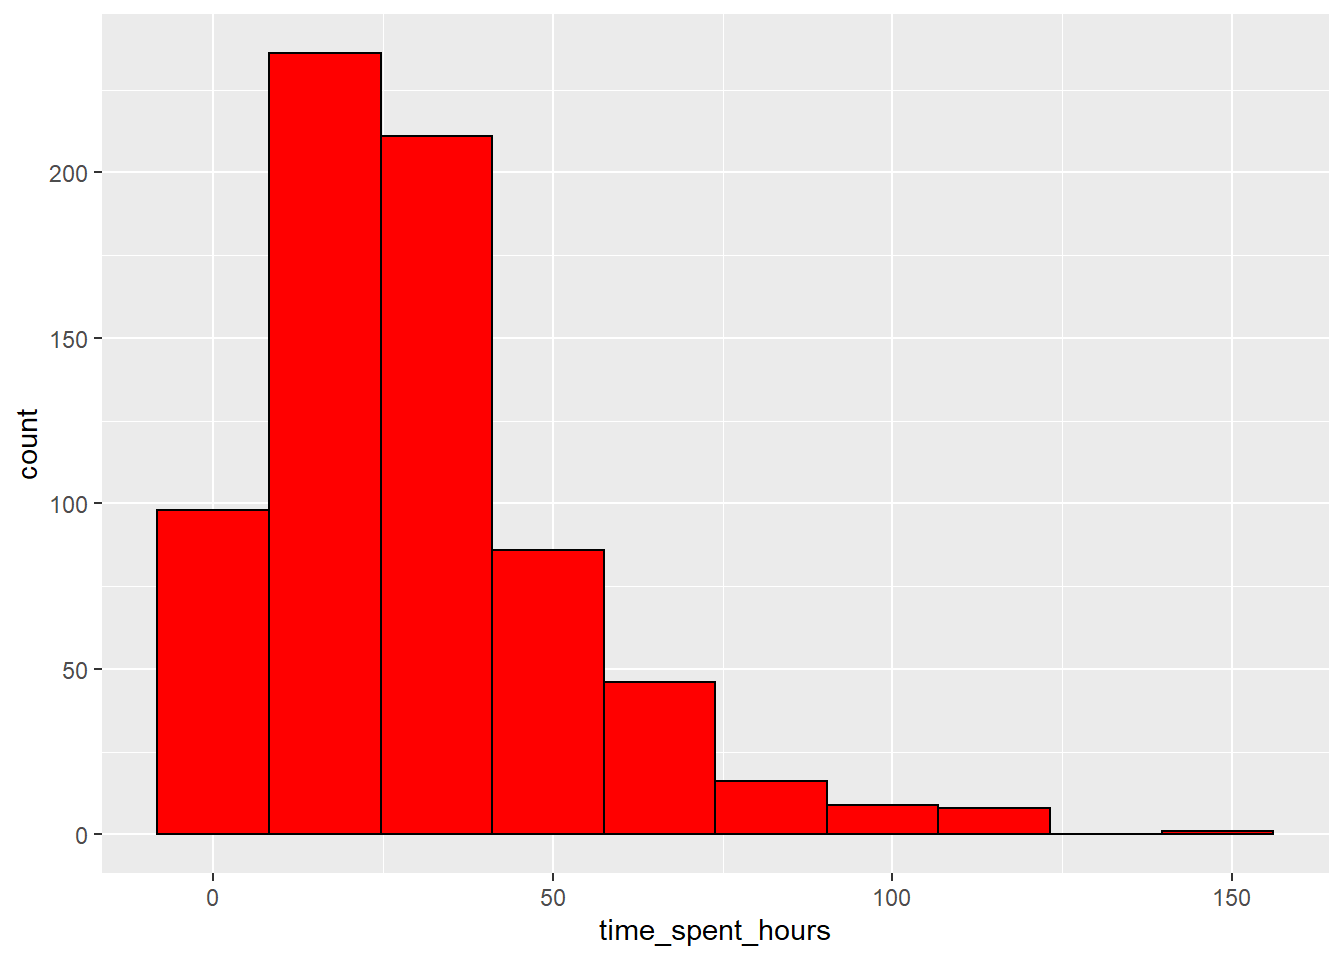
\includegraphics{final_pdf_files/figure-latex/hist3-1.pdf}

Add labels and add a theme for a clean aesthetic

\begin{Shaded}
\begin{Highlighting}[]
\CommentTok{\# Layer 1: add data and aesthetic mapping}
\NormalTok{data\_to\_explore }\SpecialCharTok{\%\textgreater{}\%} 
  \FunctionTok{ggplot}\NormalTok{(}\FunctionTok{aes}\NormalTok{(}\AttributeTok{x =}\NormalTok{ time\_spent\_hours)) }\SpecialCharTok{+}
\CommentTok{\# layer 2: add histogram geom }
\CommentTok{\# layer 3a: add bin size}
\CommentTok{\# layer 3b: add color}
  \FunctionTok{geom\_histogram}\NormalTok{(}\AttributeTok{bins =} \DecValTok{10}\NormalTok{, }\AttributeTok{fill =} \StringTok{"red"}\NormalTok{, }\AttributeTok{colour =} \StringTok{"black"}\NormalTok{)}\SpecialCharTok{+}
\CommentTok{\#layer 4: add Labels}
  \FunctionTok{labs}\NormalTok{(}\AttributeTok{title=}\StringTok{"Time Spent on LMS histogram plot"}\NormalTok{,}\AttributeTok{x=}\StringTok{"Time Spent(hours)"}\NormalTok{, }\AttributeTok{y =} \StringTok{"Count"}\NormalTok{)}\SpecialCharTok{+}
  \FunctionTok{theme\_classic}\NormalTok{()}
\end{Highlighting}
\end{Shaded}

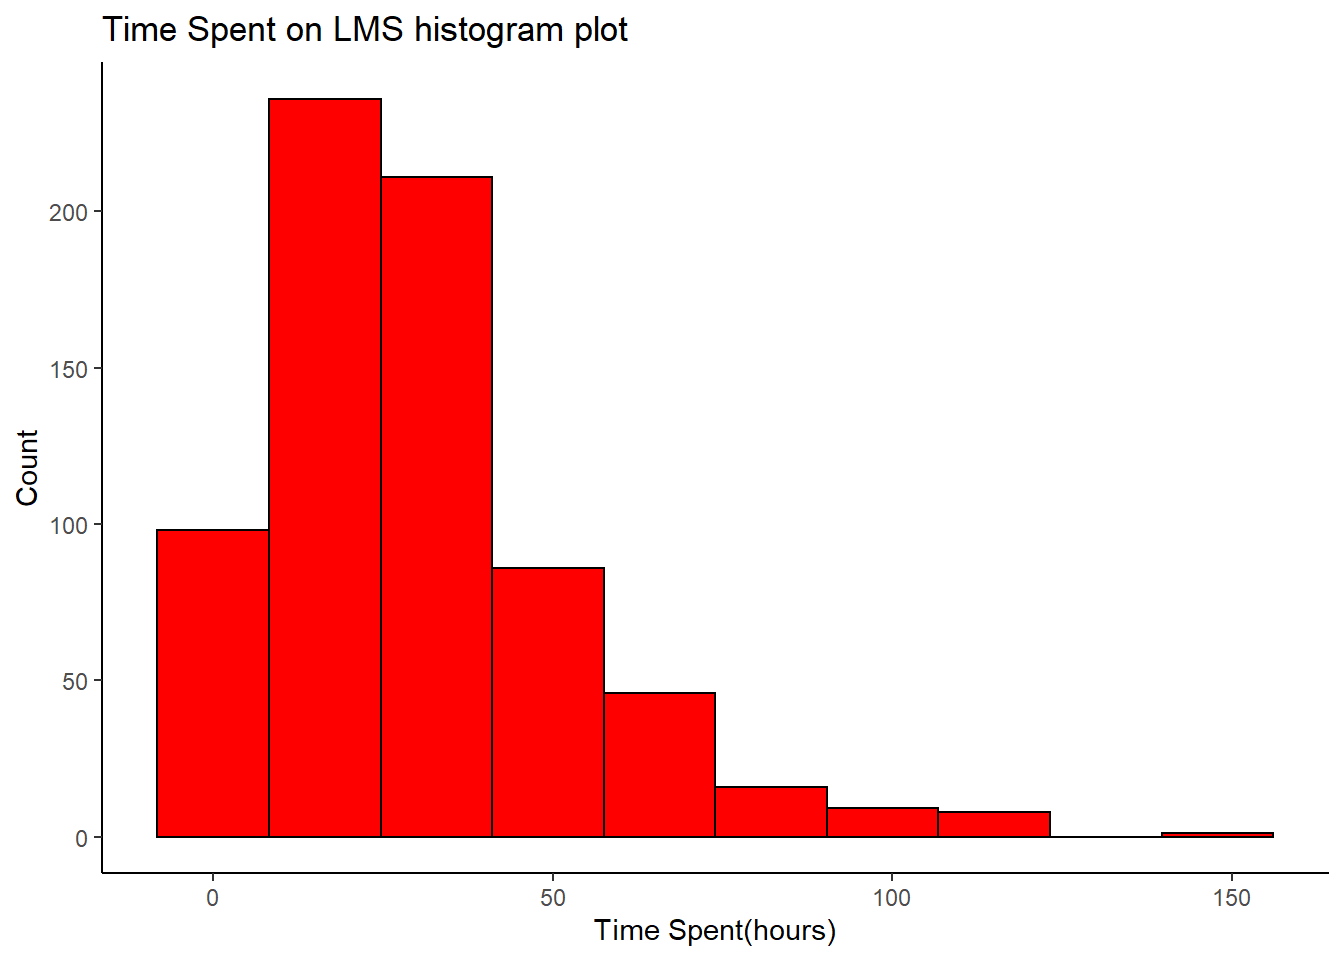
\includegraphics{final_pdf_files/figure-latex/hist4-1.pdf}

Create a histogram with density plot

\begin{Shaded}
\begin{Highlighting}[]
\NormalTok{data\_to\_explore}\SpecialCharTok{\%\textgreater{}\%}
  \FunctionTok{ggplot}\NormalTok{(}\FunctionTok{aes}\NormalTok{(}\AttributeTok{x=}\NormalTok{time\_spent\_hours)) }\SpecialCharTok{+}
  \FunctionTok{geom\_histogram}\NormalTok{(}\FunctionTok{aes}\NormalTok{(}\AttributeTok{y=}\NormalTok{..density..), }\AttributeTok{colour=}\StringTok{"black"}\NormalTok{, }\AttributeTok{fill=}\StringTok{"white"}\NormalTok{, }\AttributeTok{bins =} \DecValTok{10}\NormalTok{)}\SpecialCharTok{+}
 \FunctionTok{geom\_density}\NormalTok{(}\AttributeTok{alpha=}\NormalTok{.}\DecValTok{2}\NormalTok{, }\AttributeTok{fill=}\StringTok{"\#FF6666"}\NormalTok{) }
\end{Highlighting}
\end{Shaded}

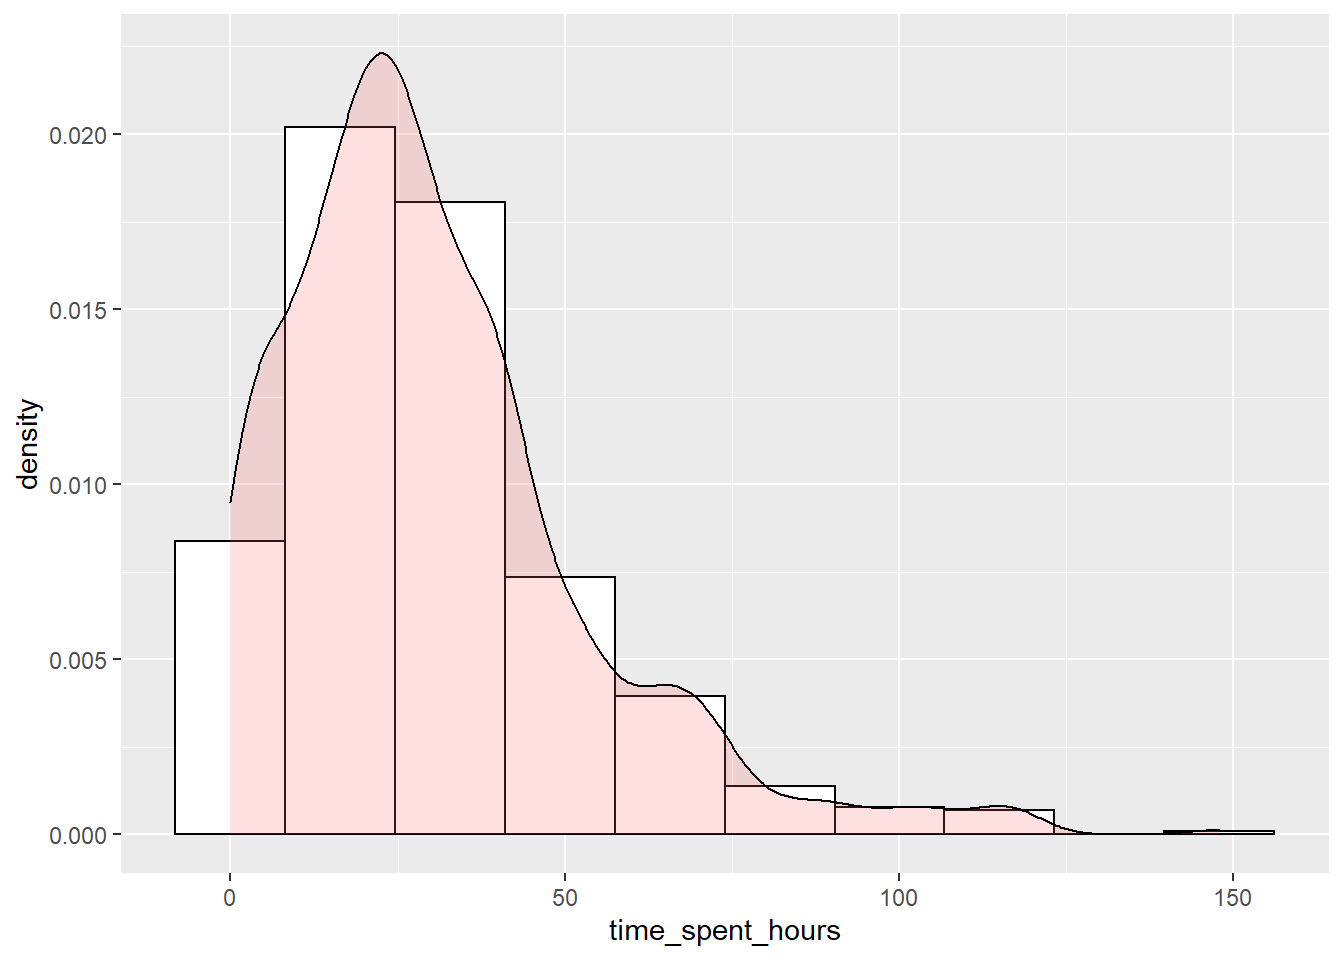
\includegraphics{final_pdf_files/figure-latex/hist5-1.pdf}

\begin{Shaded}
\begin{Highlighting}[]
  \FunctionTok{labs}\NormalTok{(}\AttributeTok{title=}\StringTok{"Time Spent on LMS histogram/density plot"}\NormalTok{,}\AttributeTok{x=}\StringTok{"Time Spent(hours)"}\NormalTok{, }\AttributeTok{y =} \StringTok{"Density"}\NormalTok{)}\SpecialCharTok{+}
  \FunctionTok{theme\_classic}\NormalTok{()}
\end{Highlighting}
\end{Shaded}

\begin{verbatim}
## NULL
\end{verbatim}

\hypertarget{model}{%
\subsection{4. Model}\label{model}}

Quantify the insights using mathematical models.

\hypertarget{a.-mathmatical}{%
\paragraph{A. MATHMATICAL}\label{a.-mathmatical}}

Does time spent predict grade earned?

\begin{Shaded}
\begin{Highlighting}[]
\CommentTok{\# Use linear regression model}
\FunctionTok{lm}\NormalTok{(proportion\_earned }\SpecialCharTok{\textasciitilde{}}\NormalTok{ time\_spent\_hours, }
   \AttributeTok{data =}\NormalTok{ data\_to\_explore)}
\end{Highlighting}
\end{Shaded}

\begin{verbatim}
## 
## Call:
## lm(formula = proportion_earned ~ time_spent_hours, data = data_to_explore)
## 
## Coefficients:
##      (Intercept)  time_spent_hours  
##         0.624306          0.004792
\end{verbatim}

\begin{Shaded}
\begin{Highlighting}[]
\CommentTok{\# Add predictor variable for science}
\FunctionTok{lm}\NormalTok{(proportion\_earned }\SpecialCharTok{\textasciitilde{}}\NormalTok{ time\_spent\_hours }\SpecialCharTok{+}\NormalTok{ int, }
   \AttributeTok{data =}\NormalTok{ data\_to\_explore)}
\end{Highlighting}
\end{Shaded}

\begin{verbatim}
## 
## Call:
## lm(formula = proportion_earned ~ time_spent_hours + int, data = data_to_explore)
## 
## Coefficients:
##      (Intercept)  time_spent_hours               int  
##         0.449657          0.004255          0.046283
\end{verbatim}

\begin{Shaded}
\begin{Highlighting}[]
\CommentTok{\# save the model}
\NormalTok{m1 }\OtherTok{\textless{}{-}} \FunctionTok{lm}\NormalTok{(proportion\_earned }\SpecialCharTok{\textasciitilde{}}\NormalTok{ time\_spent\_hours }\SpecialCharTok{+}\NormalTok{ int, }\AttributeTok{data =}\NormalTok{ data\_to\_explore)}
\end{Highlighting}
\end{Shaded}

Run a summary model for the model you just created called, \texttt{m1.}

\begin{Shaded}
\begin{Highlighting}[]
\CommentTok{\#run the summary}
\FunctionTok{summary}\NormalTok{(m1)}
\end{Highlighting}
\end{Shaded}

\begin{verbatim}
## 
## Call:
## lm(formula = proportion_earned ~ time_spent_hours + int, data = data_to_explore)
## 
## Residuals:
##      Min       1Q   Median       3Q      Max 
## -0.66705 -0.07836  0.05049  0.14695  0.35766 
## 
## Coefficients:
##                  Estimate Std. Error t value Pr(>|t|)    
## (Intercept)      0.449657   0.066488   6.763 3.54e-11 ***
## time_spent_hours 0.004255   0.000410  10.378  < 2e-16 ***
## int              0.046282   0.015364   3.012  0.00271 ** 
## ---
## Signif. codes:  0 '***' 0.001 '**' 0.01 '*' 0.05 '.' 0.1 ' ' 1
## 
## Residual standard error: 0.2142 on 536 degrees of freedom
##   (404 observations deleted due to missingness)
## Multiple R-squared:  0.1859, Adjusted R-squared:  0.1828 
## F-statistic: 61.18 on 2 and 536 DF,  p-value: < 2.2e-16
\end{verbatim}

\begin{Shaded}
\begin{Highlighting}[]
\CommentTok{\#install apaTables if this is your first time {-} do you remember how?}

\CommentTok{\#load packages}
\FunctionTok{library}\NormalTok{(apaTables)}
\CommentTok{\# use the \{apaTables\} package to create a nice regression table that could be used for later publication.}
\FunctionTok{apa.reg.table}\NormalTok{(m1, }\AttributeTok{filename =} \StringTok{"lm{-}table.doc"}\NormalTok{)}
\end{Highlighting}
\end{Shaded}

\begin{verbatim}
## 
## 
## Regression results using proportion_earned as the criterion
##  
## 
##         Predictor      b     b_95%_CI beta  beta_95%_CI sr2  sr2_95%_CI     r
##       (Intercept) 0.45** [0.32, 0.58]                                        
##  time_spent_hours 0.00** [0.00, 0.01] 0.41 [0.33, 0.48] .16  [.11, .22] .41**
##               int 0.05** [0.02, 0.08] 0.12 [0.04, 0.19] .01 [-.00, .03] .15**
##                                                                              
##                                                                              
##                                                                              
##              Fit
##                 
##                 
##                 
##      R2 = .186**
##  95% CI[.13,.24]
##                 
## 
## Note. A significant b-weight indicates the beta-weight and semi-partial correlation are also significant.
## b represents unstandardized regression weights. beta indicates the standardized regression weights. 
## sr2 represents the semi-partial correlation squared. r represents the zero-order correlation.
## Square brackets are used to enclose the lower and upper limits of a confidence interval.
## * indicates p < .05. ** indicates p < .01.
## 
\end{verbatim}

\hypertarget{communicate}{%
\subsection{Communicate}\label{communicate}}

\textbf{RQ1}: Do males outperform females in online STEM courses?

\begin{Shaded}
\begin{Highlighting}[]
\NormalTok{data\_viz }\OtherTok{\textless{}{-}}\NormalTok{ data\_to\_explore }\SpecialCharTok{\%\textgreater{}\%}
  \FunctionTok{select}\NormalTok{(subject, gender, proportion\_earned) }\SpecialCharTok{\%\textgreater{}\%}  \CommentTok{\# reduced }
  \FunctionTok{mutate}\NormalTok{(}\AttributeTok{subject =} \FunctionTok{recode}\NormalTok{(subject, }
                          \StringTok{"AnPhA"} \OtherTok{=} \StringTok{"Anatomy"}\NormalTok{,}
                          \StringTok{"BioA"} \OtherTok{=} \StringTok{"Biology"}\NormalTok{, }
                          \StringTok{"FrScA"} \OtherTok{=} \StringTok{"Forensics"}\NormalTok{, }
                          \StringTok{"OcnA"} \OtherTok{=}  \StringTok{"Oceanography"}\NormalTok{, }
                          \StringTok{"PhysA"} \OtherTok{=} \StringTok{"Physics"}\NormalTok{)) }\SpecialCharTok{\%\textgreater{}\%}
  \FunctionTok{mutate}\NormalTok{(}\AttributeTok{grade =}\NormalTok{ proportion\_earned }\SpecialCharTok{*} \DecValTok{100}\NormalTok{) }\SpecialCharTok{\%\textgreater{}\%}
  \CommentTok{\# filter(!is.na(gender)) \%\textgreater{}\%}
  \FunctionTok{na.omit}\NormalTok{() }\SpecialCharTok{\%\textgreater{}\%} \CommentTok{\# removed all NAs instead of just those for gender}
  \FunctionTok{group\_by}\NormalTok{(subject, gender) }\SpecialCharTok{\%\textgreater{}\%} \CommentTok{\# grouped by subject and gender}
  \FunctionTok{summarise}\NormalTok{(}\AttributeTok{grade =} \FunctionTok{mean}\NormalTok{(grade), }
            \AttributeTok{sd =} \FunctionTok{sd}\NormalTok{(grade))}\CommentTok{\# calculated mean and sd for grade and saved as grade again  }

  \FunctionTok{ggplot}\NormalTok{(data\_viz, }\FunctionTok{aes}\NormalTok{(}\AttributeTok{x =}\NormalTok{ subject, }\AttributeTok{y =}\NormalTok{ grade, }
                          \AttributeTok{fill =}\NormalTok{ gender)) }\SpecialCharTok{+}
  \FunctionTok{geom\_bar}\NormalTok{(}\AttributeTok{stat =} \StringTok{"identity"}\NormalTok{, }
           \AttributeTok{position =} \FunctionTok{position\_dodge}\NormalTok{()) }\SpecialCharTok{+}
  \FunctionTok{labs}\NormalTok{(}\AttributeTok{title =} \StringTok{"Do Males out{-}preform Females in online STEM courses?"}\NormalTok{,}
       \AttributeTok{caption =} \StringTok{"Online STEM course performance, why is there still a gender gap?"}\NormalTok{,}
       \AttributeTok{y =} \StringTok{"Average Grade"}\NormalTok{,}
       \AttributeTok{x =} \StringTok{"Online STEM Course"}\NormalTok{)}
\end{Highlighting}
\end{Shaded}

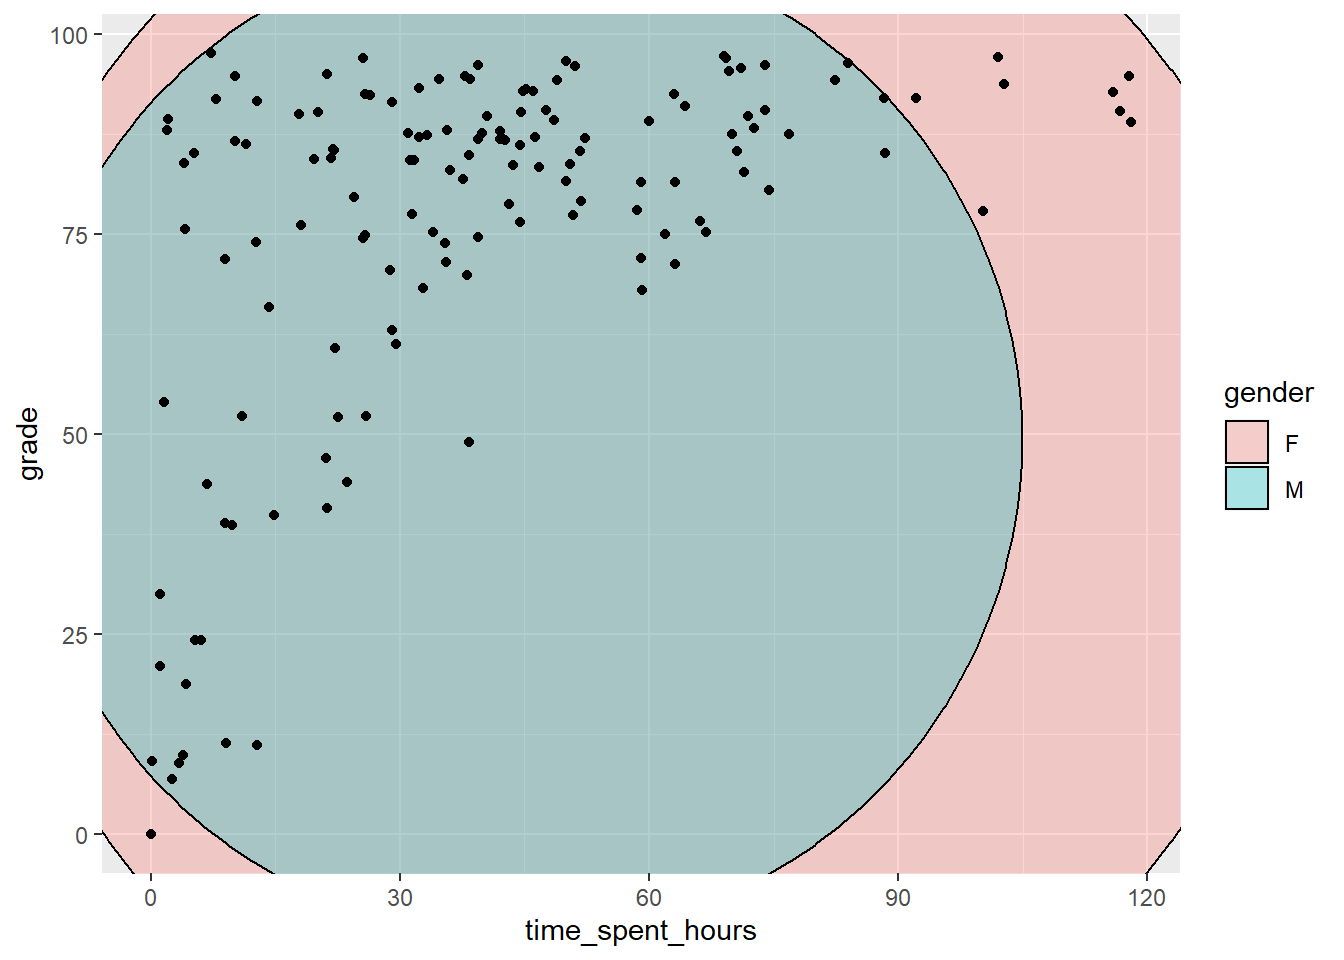
\includegraphics{final_pdf_files/figure-latex/unnamed-chunk-13-1.pdf}

\end{document}
